\chapter{Introducción}


El auge de los pequeños multirrotores no tripulados (comúnmente llamados drones) en diversos ámbitos ha crecido de forma exponencial durante estos últimos años. Se puede observar la presencia de estos drones en diversos ámbitos como: el industrial, para realizar inspecciones en lugares de difícil acceso o en lugares peligrosos, el cinematográfico, para grabar escenas aéreas, o para dispositivos de búsqueda y rescate, en los que se emplean para poder barrer grandes áreas en búsqueda de personas desaparecidas, entre otros. Además, dentro del mundo del entretenimiento las carreras de drones comienzan a hacerse un hueco en países como los Estados Unidos, donde las carreras de drones son un deporte que se retransmite en algunos canales de televisión. 

Actualmente, en la mayoría de estas competiciones, los drones están pilotados por un humano, aunque recientemente, empiezan a aparecer carreras de drones autónomos, en los que las aeronaves tienen que recorrer el circuito entero de forma autónoma sin la intervención de un humano. Algunos ejemplos de estas competiciones serían: la \textit{IROS Autonomous Drone Race}, que se celebra anualmente dentro de la conferencia de robótica internacional  IROS, o más recientemente AlphaPilot, una carrera de drones autónomos organizada por la \textit{Drone Racing League} y la empresa \textit{Lockheed Martin} con un gran premio de 1 millón de dólares para el ganador.

\begin{figure}[htb!]
	\centering
	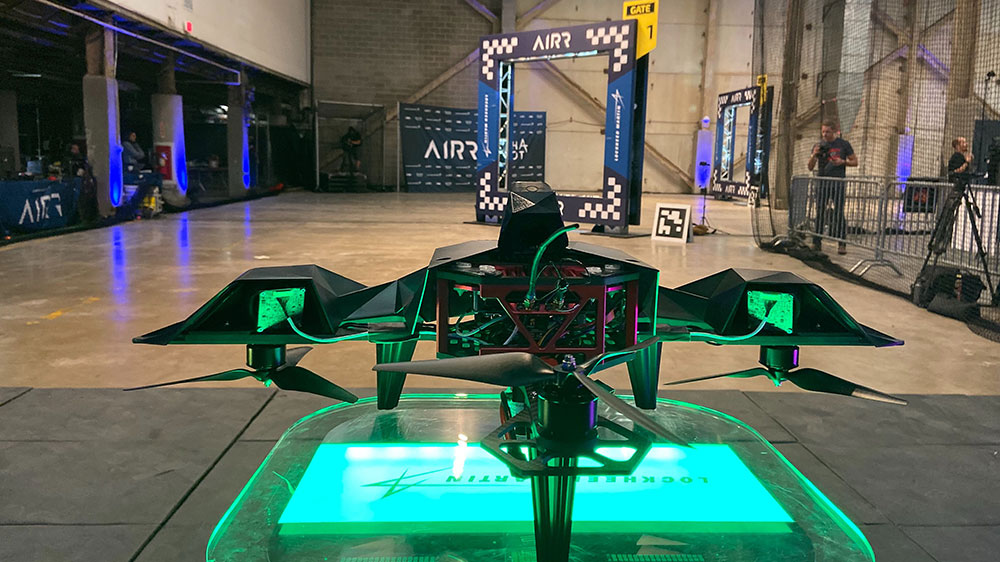
\includegraphics[width=0.80\textwidth]{imagenes/foehnAlphaPilot}
	\caption{Cuadricóptero empleado en el AlphaPilot 2019, mirando hacia la primera puerta del circuito \cite{foehn2020alphapilot}}
	\label{}
\end{figure}


Actualmente, el rendimiento obtenido por los drones de carreras autónomos aún están lejos de alcanzar el de los pilotos humanos, es por esto que el afán por superar el nivel de los pilotos humanos es una motivación para los grupos de investigación por todo el mundo. El desarrollo de drones autónomos es un campo de estudio exigente que involucra el desarrollo de la tecnología existente en diversos campos de la robótica como: la estimación, el control, la generación de trayectorias o la percepción, entre otros. 

\section{Motivación}

El desarrollo de un sistema capaz de recorrer un circuito de forma autónoma sin interacción externa con cierta incertidumbre sobre el entorno, es un problema apasionante debido a las elevadas velocidades de vuelo y la limitada capacidad computacional, que exigen tener algoritmos de percepción y de estimación de estado más precisos y rápidos, así como algoritmos de planificación y de control más rápidos y ligeros, que permitan realizar cálculos a tiempo real.

Los avances obtenidos en diversos campos de la robótica durante el desarrollo de estos drones autónomos de carreras se pueden extrapolar para mejorar el rendimiento de los drones autónomos empleados para realizar distintas tareas con una mayor relevancia como pueden ser la aplicaciones industriales o como aquellas relacionadas con la búsqueda y rescate.

Los últimos avances en las plataformas de simulación enfocadas al desarrollo de sistemas de control de drones autónomos, como el simulador fotorrealista FlightGoggles desarrollado por Guerra et al \cite{guerra2019flightgoggles} empleado durante las pruebas clasificatorias del AlhpaPilot 2019, permiten probar el rendimiento de un sistema autónomo de forma realista y segura.



\section{Solución propuesta}
El objetivo propuesto consiste en diseñar una arquitectura de un sistema modular capaz de controlar un cuadrirrotor a través de un circuito de carreras de forma autónoma.

Debido a la gran complejidad que presenta el desarrollo completo de todos los módulos que intervienen en un dron de carreras autónomo, se han simplificado el desarrollo de los módulos de estimación de estado y de percepción del circuito, empleando datos provistos por el simulador. Es por esto que el trabajo se haya centrado en el desarrollo de la arquitectura del sistema y del desarrollo de los módulos de control y generación de trayectorias capaces de generar y seguir trayectorias agresivas a lo largo de todo el circuito un circuito de carreras simulado a altas velocidades con incertidumbre sobre el recorrido en sí.

Para el algoritmo de control se han implementado dos controladores del estado del arte, un controlador para orientaciones de la aeronave con ángulos pequeños y otro para grandes ángulos, y se ha comparado el rendimiento de ambos en el seguimiento de diversas trayectorias.

En cuanto a la generación de trayectorias, se ha optado por generar trayectorias polinómicas óptimas de tipo \textit{spline}. Para poder mejorar la capacidad de reacción del aeronave ante cambios en el circuito se ha dividido la  generación de trayectorias en dos partes: la generación de una trayectoria completa a través de todo el circuito (largo plazo) y la generación de una trajectoria corta entorno a un horizonte temporal próximo a la posición del aeronave (corto plazo).

Para desarrollar los algoritmos y comparar el rendimiento del sistema realizado, se ha empleado el simulador FlightGoogles, empleado para las pruebas clasificatorias del AlphaPilot 2019 como entorno de pruebas.


%Este sistema estará formado por 3 partes principales:
%\begin{itemize}
%	\item \textbf{Estimación de estado:} Para poder recorrer el circuito es necesario tener una estimación precisa del estado de la aeronave a lo largo del tiempo. Para poder localizar el desarrollo de los 2 bloques posteriores se empleará la estimación provista por el simulador.
%	\item \textbf{}
%	\item \textbf{Generación de trayectorias:}
%\end{itemize}

\section{Objetivos}


Para poder llevar a cabo el desarrollo del trabajo de forma adecuada es conveniente desgranar los objetivos principales en tareas de alcance más reducido:

\begin{itemize}
	\item \textbf{Modulo de control}	
	\begin{itemize}
		\item Modelado dinámico del comportamiento de un cuadricóptero.
		\item Estudio del estado del arte acerca de los algoritmos de control más relevantes en las carreras de drones.
		\item Desarrollo teórico de los algoritmos de control para ángulos pequeños
		y para ángulos grandes.
		\item Implementación de ambos algoritmos dentro del módulo de control.
		\item Ajuste de los parámetros de los controladores.
		\item Evaluación del rendimiento de ambos controladores en un entorno simulado.
				
	\end{itemize}

	\item \textbf{Generación de trayectorias}	
	\begin{itemize}
		\item Estudio del estado del arte acerca de los métodos de generación de trayectorias más empleados.
		\item Desarrollo teórico de los algoritmos de generación de trayectorias que se van a emplear.
		\item División del módulo generador de trayectorias en corto y largo plazo.
		\item Implementación de los algoritmos de generación de trayectorias empleados.
		\item Evaluación del rendimiento de los generadores de trayectorias mediante el recorrido del circuito de carreras en simulación.
	\end{itemize}

	\item \textbf{Arquitectura del sistema}	
	\begin{itemize}
		\item Estudio de las arquitecturas empleadas por los ganadores de las diversas competiciones de drones autónomos.
		\item Descomposición del sistema en los distintos módulos separados que compondrán la arquitectura final.
		\item Implementación de los módulos de estimación y percepción partiendo de las mediciones provistas por el simulador.
		\item Evaluación del funcionamiento completo de la arquitectura mediante el recorrido del circuito simulado. 
		
	\end{itemize}
	
	
\end{itemize}